\documentclass[12pt,a4paper]{article}
\usepackage{url}            % clickable urls
\usepackage[T1]{fontenc}    % accents
\usepackage[utf8]{inputenc} % for non-ascii
\usepackage[autolanguage]{numprint}       % print numbers with commas etc
\usepackage{mdframed}
\usepackage[font={small,it}]{caption}

% math, symbols, fonts
\usepackage{amsthm}
\usepackage{amsmath}        
\usepackage{mathrsfs}       
\usepackage{amssymb}        
\usepackage{amsfonts}       

%layout
\usepackage{subfig}
\usepackage{geometry}       % layout tables and figures automagically
\usepackage[table]{xcolor}
\usepackage{colortbl}

%drawing
\usepackage{pgf}
\usepackage{tikz}
\usetikzlibrary{arrows,automata,positioning,calc,svg.path}
\usepackage[compat=1.1.0]{tikz-feynhand}

\usepackage[texcoord=true]{eso-pic}
\usepackage{hyperref}
\usepackage{todonotes}

\AddToShipoutPictureBG{
 \AtStockUpperLeft{
 \hspace{1cm}
 \begin{tikzpicture}[baseline=(k.base)]
\begin{feynhand}
\vertex (k) at (1,3);
\vertex (a) at (0.125,-1); 
\vertex (b) at (-1,0); 
\vertex (c) at (0.875,2);
\vertex (d) at (2,1) {};
\vertex [dot, gray] (o) at (0,0) {}; 
\vertex [dot, gray] (p) at (1,1) {}; 
\propag [fermion, gray] (o) to (a);
\propag [fermion, gray] (b) to (o); 
\propag [glu, gray] (o) to (p);
\propag [fermion, gray] (c) to (p);
\propag [fermion, gray] (p) to (d);
\end{feynhand}
\end{tikzpicture}
 }
}
 
\hypersetup{
  colorlinks   = true,    % Colours links instead of ugly boxes
  urlcolor     = blue,    % Colour for external hyperlinks
  linkcolor    = blue,    % Colour of internal links
  citecolor    = red      % Colour of citations
}

\newcommand*{\svgat}{%
  \leavevmode
  \tikz[baseline=0pt, x=1pt, y=1pt, scale=1em/1000]\fill
    svg {
      M588 457v-241c0 -15 0 -66 35 -66c66 0 73 90 73 182c0 241 -171 351 -308
      351c-164 0 -307 -145 -307 -336c0 -179 130 -336 312 -336c94 0 187 24
      272 64c5 3 7 3 23 3h9c16 0 23 0 23 -10c0 -16 -120 -51 -146 -57c-64 -15
      -128 -22 -180 -22 c-200 0 -338 170 -338 358c0 199 150 358 333 358c161
      0 332 -133 332 -367c0 -107 -14 -210 -102 -210c-38 0 -90 19 -100 71c-30
      -42 -78 -71 -132 -71c-103 0 -198 93 -198 219s95 219 198 219c39 0 91
      -14 137 -77c6 -7 7 -8 23 -8h17c23 0 24 -1 24 -24zM519 262v170 c0 18 0
      21 -13 40c-36 56 -84 72 -116 72c-73 0 -132 -86 -132 -197s60 -197 132
      -197c20 0 71 6 115 69c14 21 14 25 14 43z
    }
    (current bounding box.west) ++(-56, 0) % left side bearing
    (current bounding box.east) ++(56, 0) % right side bearing
  ;%
}

\newcommand*{\svgperiod}{%
  \leavevmode
  \tikz[baseline=0pt, x=1pt, y=1pt, scale=1em/1000]\fill
    svg {
      M192 53c0 -29 -24 -53 -53 -53s-53 24 -53 53s24 53 53 53s53 -24 53 -53z
    }
    (current bounding box.west) ++(-86, 0) % left side bearing
    (current bounding box.east) ++(85, 0) % right side bearing
  ;%
}

\title{Gluon Plasma \\
\large A Plasma Variant for Non-custodial Exchanges}

\author{Bharath Rao \\ 
Leverj\\
bharath\svgat leverj\svgperiod io \\
\tiny WORKING DRAFT}

\newcommand{\question}[2]{\todo[inline,author=#1]{#2}}
\newcommand{\reponse}[2]{\todo[inline,color=green,author=#1]{#2}}


\begin{document}

\maketitle

\begin{abstract}

        We introduce a plasma sidechain designed specifically for non-custodial, high-speed, low-latency trading. We explore extending the value proposition of plasma to a financial institution using comprehensive set of fraud-proofs to enforce correctness and voting to handle data unavailability. We describe a hybrid DEX that enables us to trade at high-speed, at low gas cost, and with support for fast withdrawals without handing over funds custody to the sidechain operator. 
\end{abstract}
\section{Introduction}

The largest use case of cryptocurrencies is trading, which is currently dominated by centralized exchanges. Users who trade on centralized exchanges tolerate custodial risk for the benefits of low-latency and high-speed trading. We aim to break this dichotomy and present a protocol that enables low-latency, high-speed trading without custodial risks. 
Sidechain models such as plasma allow us to leverage the benefits of blockchain while using only a small footprint on the main chain. We introduce a flavor of plasma designed especially for exchanges to enable trustless non-custodial trading.

\section{Previous Work}

Nakamoto’s breakthrough innovation, Bitcoin\cite{Nak09} made trustless transactions feasible and triggered the cryptocurrency boom that is likely still in its infancy. A currency whose rules are impractical to break even for state actors has triggered thousands of projects that hope to leverage its underlying blockchain technology to create self-compliant systems. 
Ethereum\cite{Eth14} extended the blockchain into a Turing-complete world computer. This was formalized in Gavin Wood’s seminal yellow paper\cite{Gav15}. Ethereum became the platform of choice for smart contracts that have generalized state and logic. Plasma\cite{PB17} enables a high transaction rate using a sidechain with safe exit to the main chain. Multiple flavors of plasma exist, with various tradeoffs between user burden, speed and convenience.

\section{Trustless Finance}

The appeal of cryptocurrency is its ability to self-regulate and confirm with its internal consensus rules without the need of a centralized enforcer. This has been variously characterized as being \emph{permissionless, decentralized} or \emph{trustless}. 

What exactly makes something trustless? A system is trustless if all assets are always in the custody of their owners, transfers do not need a trusted intermediary and the integrity of all asset transfers can be verified by network participants with certainty.

The above definition translates to the following four constraints\footnote{Appendix \ref{app:safety} explores these in detail.}:
\begin{enumerate}
    \item \emph{Segregation:} Coins are created or sent directly into the owner’s custody. 
    \item \emph{Agency:} Coin ownership can only change with the provable intention of the owner.
    \item \emph{Solvency:} Only legitimately created and previously unspent coins can be spent.
    \item \emph{Integrity:} Coin movement should comply with all network consensus rules\footnote{Consensus rules modeled as constraints:                             \url{https://en.bitcoin.it/wiki/Protocol_rules}}.
\end{enumerate}
Segregation enforces self-custody and removes the need for trusted third parties. Agency enables tracing a coin’s provenance to its creation. Solvency ensures that the scarcity and value are preserved. Integrity ensures that reliable coin transfer can be verified by observers. All four combined enable the creation of a trustless value network. 

While solvency may superficially appear to be simply another integrity constraint, it is different in an important aspect. Most integrity violations can be detected immediately from an examination of the transaction bytes, leading to the rejection of the associated transaction. Solvency (i.e., double-spend protection) is handled differently as it requires a conflicting transaction to invalidate an otherwise valid transaction. Nakamoto consensus\cite{nakcons} eventually resolves any solvency issues in Proof-of-work (POW) blockchains\cite{DN93}. It is important to address solvency correctly in Proof-of-Authority (POA)\cite{parPOA} systems to avoid catastrophic losses.

\subsection{A Graph-Theoretic Model of a Trustless UTXO System}
We represent addresses holding coins using nodes in a graph and movements of coins as directed edges. In an unspent transaction output system, coins can be merged and split in a transaction and every transaction output is a separate coin that needs to be spent with a separate signature. An output therefore is an inbound edge into an address.

\begin{figure}[ht]
\begin{center}

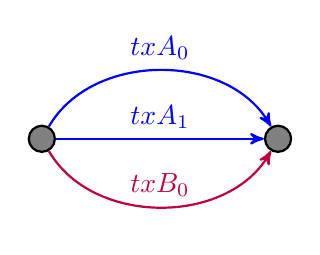
\begin{tikzpicture}[->,>=stealth',auto,node distance=3cm,
  thick,main node/.style={circle,draw,font=\sffamily\Large\bfseries}]

  \node[main node,fill=gray] (1) [] {};
  \node[main node,fill=gray] (2) [right of=1] {};

  \path[every node/.style={font=\sffamily}]
    (1) edge [blue,bend left=60] node [above] {$txA_0$} (2)
    (1) edge [blue] node [above] {$txA_1$} (2)
    (1) edge [purple,bend right=60] node [above] {$txB_0$} (2);
\end{tikzpicture}

\end{center}
\caption{The same address may hold unspent outputs from multiple transactions. The address on the right holds two UTXOs from txA and one from txB}
\end{figure}

A new transaction can spend multiple unspent outputs from different transactions and distribute them to multiple recipients\cite{Max13}. A transaction can be validated by checking that outputs are sent directly to the recipient (\emph{Segregation}), all spent inputs are signed (\emph{Agency}), only valid unspent balances are spent (\emph{Solvency}) and the transaction complies with all consensus rules (\emph{Integrity}). Once these rules are validated for each UTXO, they can all be marked as verified edges. 

In UTXO networks, coins are created into the control of the owner. For example, the bitcoin network’s coinbase transaction creates block reward coins going from \emph{Origin}\footnote{Bitcoin uses the UTXO with transaction Id 0, Output index -1 to denote the \emph{Origin}\cite{BTCProtocol}.} into the owner’s address. 
\begin{figure}[ht]
\begin{center}
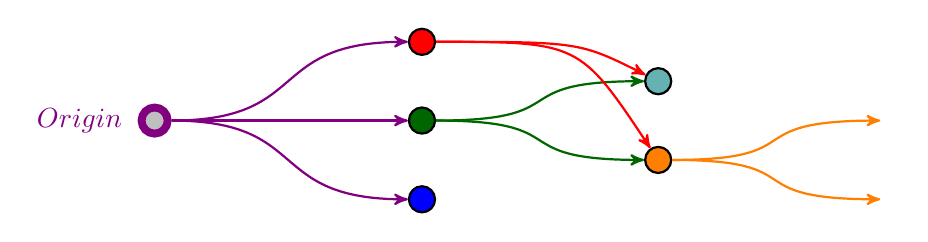
\begin{tikzpicture}[->,>=stealth',auto,node distance=3cm,
  thick,main node/.style={circle,draw,font=\sffamily\Large\bfseries}]
  
  \node[main node,violet,line width=1mm,fill=lightgray,anchor=east] at (0,0) (o) {};
  \node[anchor=east,violet] at (-0.5,0) (x) {$Origin$};
  \node[main node,fill=red,anchor=west] at (3,1) (a) {};
  \node[main node,fill=black!60!green,anchor=west] at (3,0) (b) {};
  \node[main node,fill=blue,anchor=west] at (3,-1) (c) {};
  \node[main node,fill=teal!60,anchor=west] at (6,0.5) (d) {};
  \node[main node,fill=orange,anchor=west] at (6,-0.5) (e) {};
  \node[anchor=west] at (9,0) (f) {};
  \node[anchor=west] at (9,-1) (g) {};
  \draw[->,violet] (o) .. controls ([xshift=2cm] o) and ([xshift=-2cm] a) .. (a);
  \draw[->,violet] (o) .. controls ([xshift=2cm] o) and ([xshift=-2cm] b) .. (b);
  \draw[->,violet] (o) .. controls ([xshift=2cm] o) and ([xshift=-2cm] c) .. (c);
  \draw[->,black!60!green] (b) .. controls ([xshift=2cm] b) and ([xshift=-2cm] d) .. (d);
  \draw[->,black!60!green] (b) .. controls ([xshift=2cm] b) and ([xshift=-2cm] e) .. (e);
  \draw[->,red] (a) .. controls ([xshift=2cm] a)  .. (d);
  \draw[->,red] (a) .. controls ([xshift=2cm] a)  .. (e);
  \draw[->,orange] (e) .. controls ([xshift=2cm] e) and ([xshift=-2cm] f) .. (f);
  \draw[->,orange] (e) .. controls ([xshift=2cm] e) and ([xshift=-2cm] g) .. (g);
\end{tikzpicture}

\end{center}
\caption{UTXOs as validated paths flowing from origin transaction to addresses }
\end{figure}

An UTXO model’s safety can be modeled as a valid path in a directed graph. 
An UTXO is valid if and only if there is a verified path to it from origin: 
\begin{enumerate}
    \item An unbroken chain of signatures (agency)
    \item to the origin transaction (segregation) 
    \item of valid consensus confirming transfers (integrity and solvency)
\end{enumerate}
Verification is onerous in a large graph. Since coins are split in most transactions, it’s not sufficient to do a breadth-first search. Rather, all inputs of every transaction that participates in the path should be verified as valid. This rapidly becomes a large set with every new transfer, similar to a human’s list of ancestors. The number of potential paths is very large, so blockchains amortize validation by downloading every transaction and verifying them as they are added. This allows us to assume that every reference to an already verified transaction is a valid path and only verify the most recently added UTXOs.

\section{Exchange Security Models}
\subsection{Centralized Exchanges}
Custody and ownership are intertwined and transferred together in an UTXO coin, but centralized exchanges split the two concerns. A user gives up custody to the exchange when he deposits coins into his deposit address but retains ownership.
\begin{figure}[ht]
\begin{center}
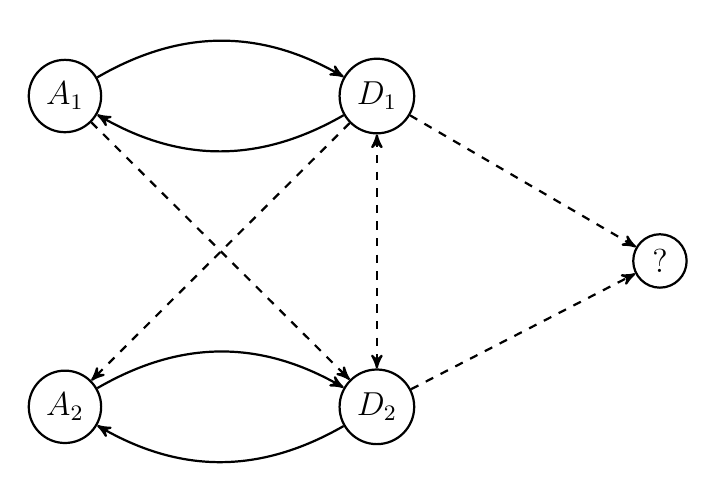
\begin{tikzpicture}[->,>=stealth',auto,node distance=30mm,
  thick,main node/.style={circle,draw,font=\sffamily\large\bfseries}]
    \node[main node](A1){$A_1$};
    \node[main node,below=of A1](A2){$A_2$};
    \node[main node,right=of A1](D1){$D_1$};
    \node[main node,right=of A2](D2){$D_2$};
    \node[main node,below right=15mm and 30mm of D1](X){\large $?$};
    \path (A1) [bend left] edge (D1)
          (D1) [bend left] edge (A1)
          (A2) [bend left] edge (D2)
          (D2) [bend left] edge (A2)
    ;
    \path[<->]
          (D1) [dashed] edge (D2)
    ;
    \path
          (A1) [dashed] edge (D2)
          (D1) [dashed] edge (A2)
          (D1) [dashed] edge (X)
          (D2) [dashed] edge (X)
    ;
           
\end{tikzpicture}

\end{center}
\caption{Centralized exchange showing no constraints on funds movement among user addresses $A_i$ and deposit addresses $D_i$, rendering security proofs infeasible. }
\end{figure}

 This situation gives rise to the chances of someone else losing your coins through malice or general incompetence. Exchanges try to limit this risk by splitting their holdings into a majority cold wallet\cite{BTCColdStorage} and minority hot wallet holdings. The cold wallet custody is vested among a small set of trusted officers to reduce risk of theft.

Centralized exchanges have no security properties since none of the four constraints are enforced. Segregation does not exist, since depositing involves essentially giving up custody to the operator; and anyone can deposit coins into any account or withdraw to any address enabling phishing attacks. 

Without self-custody, there is no agency. However, an exchange may simulate agency via associated side channels such as email confirmations or two-factor authentication (2FA). Ultimately, all side channel verifications boil down to an identity check plus association of the identity with the account. This interface is not seamless and provides for a variety of attacks. Intertwined identity and agency using crypto addresses and signatures are stronger than any mobile 2FA side channel association and authentication\cite{DLRS14}. 

There is no simple way to prove solvency of user funds continuously. Even with periodic proof-of-reserves, there is no way for the exchange to prove that it’s not running a fractional reserve since there is no solvency constraints for withdrawals or other transactions. Consequently, theft is often not detected for quite some time and often operators may lose user funds in risky ventures without anyone’s knowledge.

The absence of publicly verifiable integrity checks eliminates any practical way to prove the invalidity of balance changes caused by maleficent operators or random bugs in the exchange code. This situation enables exchanges to engage in or turn a blind eye to all manner of manipulation; for example, giving friends the ability to place large orders without funds backing such orders.

In summary, all major exchange problems are a result of their inability to enforce the four trustless constraints. We believe this is true for all other financial systems that may be built on smart contract capable blockchains.

\subsection{On-chain Exchanges (DEX)}
\begin{figure}[ht]
\begin{center}

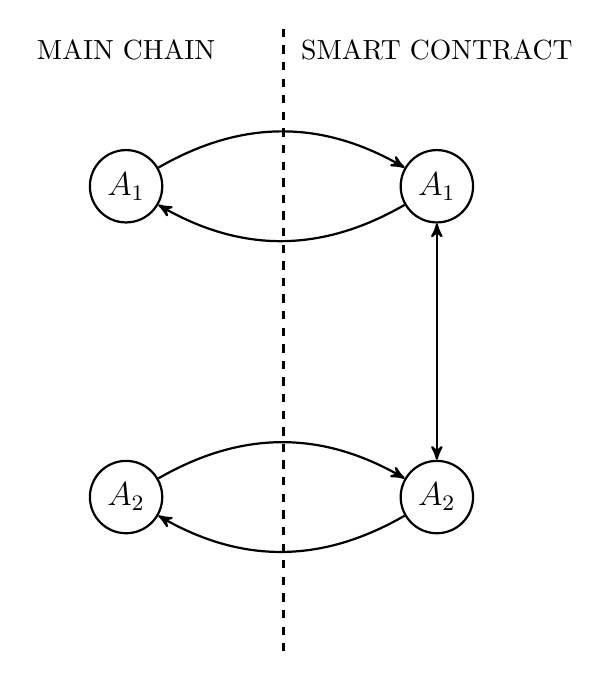
\begin{tikzpicture}[->,>=stealth',auto,node distance=3,
  thick,main node/.style={circle,draw,font=\sffamily\large\bfseries}]
    \node[main node](A1){$A_1$};
    \node[main node,below=of A1](A2){$A_2$};
    \node[main node,right=of A1](D1){$A_1$};
    \node[main node,right=of A2](D2){$A_2$};
    \node[above=1 of A1]{MAIN CHAIN};
    \node[above=1 of D1]{SMART CONTRACT};
    \path (A1) [bend left] edge (D1)
          (D1) [bend left] edge (A1)
          (A2) [bend left] edge (D2)
          (D2) [bend left] edge (A2)
    ;
    \path[<->]
          (D1) edge (D2)
    ;
    \draw[-,dashed] (2,2) -- (2,-6);

\end{tikzpicture}

\end{center}
\caption{On-chain exchanges provide safety by syncing every transaction to the blockchain but are constrained on scale and latency. }
\end{figure}
On-chain exchanges can enforce the above constraints quite easily since interacting with the network and posting a blockchain transaction do most of the heavy lifting.
The early decentralized exchanges models are fully on-chain, i.e., they use a smart contract to hold order books or reserves of tokens that users can interact with to perform trades. Naturally, the per transaction costs of such exchanges are very high and latency is limited by blockchain speeds, usually at intolerable levels. Such exchanges are also susceptible to a variety of front-running and DOS attacks\cite{levprotocol}.

\subsection{Hybrid Exchanges}
A hybrid exchange uses a smart contract to hold user funds and enables trustless trades between participants facilitated by a centralized entity. Although this can be a lot faster since orders don’t need to go into the contract until filled, proving safety is a bit more involved\cite{levprotocol}. 

Since the smart contract can identify the source address and the network has already verified the user signature, its trivial to credit deposited funds directly into the custody of the sender, making enforcement of the segregation constraint straight forward --- the operators of the exchange never take custody of funds. 

This scheme also facilitates solvency checks ensuring that the exchange is never at fractional reserve. The integrity checks are a bit more involved and require proving orders and fills are unique, have not been replayed and there are no race conditions between fills and cancels. This is accomplished by storing filled and cancelled orders or execution in the contract resulting in high costs and low speeds\cite{WA17}. In addition, price-time priority proofs need to be added to verify that the exchange is not skimming the users.

\section{Plasma and Plasma Exchanges}
One way to dramatically reduce on-chain cost and improve latencies is to use a specialized sidechain to execute trades and perform settlements. This would reduce the main-chain footprint to deposits, withdrawals and occasional commitment of state integrity to the main chain. Plasma as a sidechain on Ethereum is the most advanced option as of this writing.

\subsection{Plasma Classic Outline}
The original idea of plasma (Plasma Classic) has blossomed into multiple flavors to suit the needs of various projects, but the central idea is essentially the same\footnote{Originally posted at: \url{https://ethresear.ch/t/plasma-classic-compact-spec/1711}}: \emph{The sidechain is valid as long as all changes on it are verifiable. There is a way to safely exit when the sidechain is no longer verifiable}.

\begin{enumerate}
    \item A plasma sidechain $P$ is anchored to root chain $R$
    \item A deposit in $R$ creates UTXO in $P$
    \item A withdrawal from $R$ removes UTXO from $P$
    \item State changes in $P$ are periodically committed into $R$ as block headers.
    \item Block headers contain sufficient information to prove correctness of state transitions
    \item Incorrect state transitions in $P$ are rolled back (up to a point) using fraud-proofs on $R$
    \item Exits are prioritized by earlier $P$ blocks, to ensure fraudulent outputs fail
    \item If information needed for fraud-proofs is withheld, mass exit from $P$ to $R$
\end{enumerate}

\subsection{Plasma Exchange}
\begin{figure}[ht]
\begin{center}

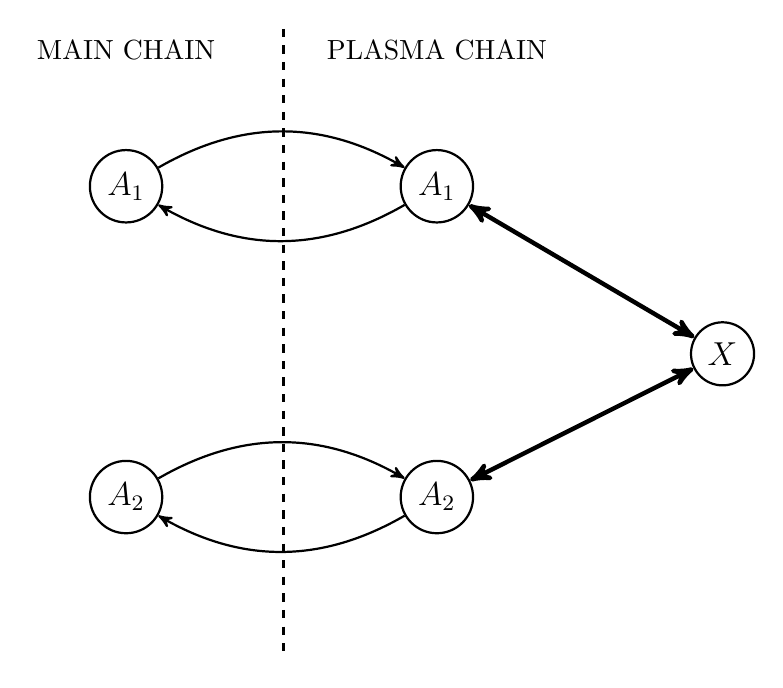
\begin{tikzpicture}[->,>=stealth',auto,node distance=3,
  thick,main node/.style={circle,draw,font=\sffamily\large\bfseries}]
    \node[main node](A1){$A_1$};
    \node[main node,below=of A1](A2){$A_2$};
    \node[main node,right=of A1](D1){$A_1$};
    \node[main node,right=of A2](D2){$A_2$};
    \node[main node,below right=15mm and 30mm of D1](X){$X$};
    \node[above=1 of A1]{MAIN CHAIN};
    \node[above=1 of D1]{PLASMA CHAIN};
    \path (A1) [bend left] edge (D1)
          (D1) [bend left] edge (A1)
          (A2) [bend left] edge (D2)
          (D2) [bend left] edge (A2)
    ;
    \path[<->]
          (D1) [ultra thick] edge (X) 
          (D2) [ultra thick] edge (X)
    ;
    \draw[-,dashed] (2,2) -- (2,-6);

\end{tikzpicture}

\end{center}
\caption{Plasma exchanges use smart contracts to enforce integrity without syncing trades to the main chain, combining centralized performance and decentralized safety. }
\end{figure}

The plasma exchange can scale up to the speed of centralized exchanges by avoiding the need to sync trades and orders onto the on-chain smart contract. The main-chain plasma contract that holds custody of user funds at any time has no knowledge of the exact balance of any user. It’s the responsibility of the user to provide proof-of-solvency for withdrawals. In interactive plasma variants, the user may have to post a bond that would be forfeited in case of a successful challenge by another network participant.

The proof of safety of the plasma exchange rests on the proof that the exchange can enforce \emph{Segregation, Agency, Solvency} and \emph{Integrity} in all of its operations in a manner verifiable by all participants. 

\subsection{UTXO Based Plasma Issues for Exchanges}
\begin{enumerate}
    \item \emph{Witness Baggage.} Agency (ownership) is proved by signatures going back to the main-chain deposit transaction. This list can get very large in an exchange with high volume.
    \item \emph{Onerous Ownership.} User is required to regularly check transactions on plasma sidechain for fungible coins or main chain for non-fungible coins.
    \item \emph{Stampede to Exit.} The huge number of UTXOs that need to exit on data unavailability suggest that the actual mechanics of exiting  cannot be reliably modeled due to unpredictable congestion and fees. There is a good chance that if disaster strikes, orderly exit may be impractical.
    \item \emph{UTXO Shredding.} This is the tendency of an UTXO based system to fragment  all outputs to the smallest possible size. This is a serious scalability limitation for exchanges. This is a natural outcome of price-time priority matching. Orders are matched by best price, followed by best time of order placement. Order matches will generate a partial match for the larger sized order and a full match for the smaller size order. The exchanged assets will be received in smaller outputs with every future match and this process will repeat over time resulting in each user holding a large number of smaller and smaller outputs. This amplifies the load on the sidechain even more dramatically. 
\end{enumerate}

We believe UTXO model sidechains scale poorly for exchanges and therefore have constructed an account model sidechain.

\section{Gluon Plasma}
We introduce a variant of plasma that is designed for high speed trading engines and avoids the issues of UTXO based plasma. Our plasma sidechain is designed with the following goals in mind:
\begin{enumerate}
    \item Account based
    \item Small footprint
    \item Instant finality 
    \item Fast withdrawals
    \item Compact fraud-proofs for every transition
    \item Non-Onerous safety 
    \item Congestion tolerant
    \item Incentive balanced
    \item Chain halt on data unavailability
\end{enumerate}
The custody of users’ assets on the plasma sidechain is managed by the Gluon plasma contract. The plasma contract serves as the interface for assets between the main chain and the plasma sidechain. 

The plasma contract also accepts fraud proofs and enforces correctness. Any proof of operator compromise may be submitted to the plasma contract which results in an immediate halt of the sidechain enabling withdrawal of funds at leisure. The plasma contract also enforces a chain halt to address data unavailability.

All other features not relating to custodial issues are not a concern for the plasma contract, enabling products that use the plasma sidechain to add features without the need to redeploy a new contract.
\subsection{Gluon Plasma Outline}
\begin{enumerate}
    \item Gluon plasma starts with a known zero state where all balances are zero.
    \item Deposits to the main chain of an asset by user increase the user’s asset balance on the plasma sidechain by a corresponding amount. 
    \item Withdrawing funds from the plasma sidechain decrease the balance on the sidechain and enables withdrawal on the main chain.
    \item Transfer of assets (trading) between users on the plasma sidechain require matching signed orders of the users, countersigned by the operator. 
    \item All state changes require accompanying witnesses. Any invalid witness can be used to halt the plasma sidechain and let users withdraw at leisure. 
    \item In the event of data unavailability, participants can vote to halt the sidechain, enabling users to withdraw on the main chain at leisure.
\end{enumerate}

\subsection{The Gluon Plasma Ledger}
All state changes in the plasma sidechain are recorded in a ledger that enables verification of the provenance and validity of every single balance.
\begin{enumerate}
    \item The plasma sidechain state is maintained on its own ledger. The plasma sidechain starts with a known zero state, where all balances are zero. This is reflected by a special ledger entry called the $Origin$. 
    \item Every state change creates a new ledger entry retaining a link to the prior entry that it invalidates. 
    \item Every new ledger entry enforces trustless constraints of \emph{Segregation, Agency, Solvency} and \emph{Integrity}, whose validity can be independently verified by network participants. 
    \item Every ledger entry is signed by the operator. This reflects the fact that the operator is signing off on the changes.
    \item The plasma contract will accept invalid entries signed by the operator as a fraud proof.
    \item Deposits in the main chain create a new ledger entry that reflects the user’s increased asset balance. 
    \item Ledger Entries are periodically committed to the main chain via Merkle roots. Each set of such transactions is called a \emph{Gluon Block} or \emph{G-block}. No transactions can be skipped or reordered. 
    \item All acceptable deposits occurring in a G-block are committed as an ordered Merkle root. 
    \item All current  balances of each Account/Asset pair are committed as a Merkle root.
    \item The plasma contract enforces a minimum number of main chain blocks between each G-Block to ensure sufficient latency for a vote to halt. 
    \item The last committed G-block is said to be \emph{unconfirmed} and cannot be used to initiate a withdrawal. It is open to challenges from validators. Once a newer G-Block is committed, the prior G-Block is deemed \emph{confirmed} and may be used to withdraw funds.
    \item Withdrawing some of the balance on the plasma sidechain reduces the asset balance on the sidechain and enables withdrawal from the main chain. This creates a corresponding ledger entry to reflect the reduced asset balance.
\end{enumerate}

\subsection{Ledger Entries}
Each state change is recorded in a ledger entry that includes the following:

\begin{table}[ht]
\caption{Ledger Entry fields in Gluon Plasma}
\centering
\begin{tabular}{|l|l|}
\hline
\bfseries    Field & \bfseries Meaning \\
\hline
    Entry ID &ID for the new state \\
    Prior Entry	& Prior state \\
    Type &	Origin, Deposit, Trade, Fee, Withdraw, Exited \\
    Account &	Ethereum public address of owner \\
    Asset &	Token Address. All zeros for Ethereum \\
    Quantity &	Net Change from prior balance \\
    Balance	 & New balance \\
    Witness	& Acceptable Proof of validity \\
\hline
\end{tabular}
\end{table}

\subsection{Ledger Entry types}
There are six ledger entry types: $Origin$, $Deposit$, $Withdraw$, $Exited$, $Trade$ and $Fee$.
The initial state, also known as $Origin$, is a special entry that records a universal zero balance. 

The $Deposit$ and $Withdraw$ entries are on and off ramps into the plasma contract. They increase and decrease the balance respectively. The $Exited$ entry type represents a permanent cessation of all activity for an \((Account, Asset)\) pair and reduces balance to zero. $Trade$ represents a trade of an asset pair between two accounts. $Fee$ represents fees paid to the operator.

\subsection{State Transitions}

\begin{table}[ht]
\caption{Ledger Entry fields in Gluon Plasma. Account data are signed by the account private key and entries by operator key. The symbol $*$ indicates "any."}
\centering
\begin{tabular}{|c|c|c|c|c|r|r|c|}
\hline

\bfseries State &\bfseries  Prior &\bfseries  Type &\bfseries  Account &\bfseries  Asset &\bfseries  Qty. &\bfseries  Bal. &\bfseries  Witness  \\
\hline
0 & 0 & Origin & $*$ & $*$ & 0.00 & 0.00 &  \\
1 & 0 & Deposit & $A_1$ & $Z_1$ & $+0.10$ & 0.10 & Deposit Hash  \\
2 & 1 & Trade & $A_1$ & $Z_1$ & $-0.05$ & 0.05 & Orders, Fill \\
3 & 0 & Trade & $A_1$ & $Z_2$ & $+0.02$ & 0.02 & Orders, Fill \\
4 & 3 & Withdraw & $A_1$ & $Z_2$ & $-0.01$ & 0.01 & Prior balance \\
5 & 4 & Exited & $A_1$ & $Z_2$ & $-0.01$ & 0.00 & Exit Block \\
\hline
\end{tabular}
\label{sampleEntries}
\end{table}

Every state transition has sufficient witness data to prove correctness of the new entry and a link to the prior entry. A partial set of entries for an account $A_1$ that deposits asset $Z_1$ and trades 0.05 of it for 0.02 of Asset $Z_2$ and finally withdrawing and exiting is shown in Table \ref{sampleEntries}.

Note that $state_{2}$ obsoletes $state_1$ for the tuple \((A_1, Z_1)\) but $state_3$ is a new state for \((A_1, Z_2)\), therefore its prior entry points to $Origin$.

\begin{figure}[ht]
\begin{center}
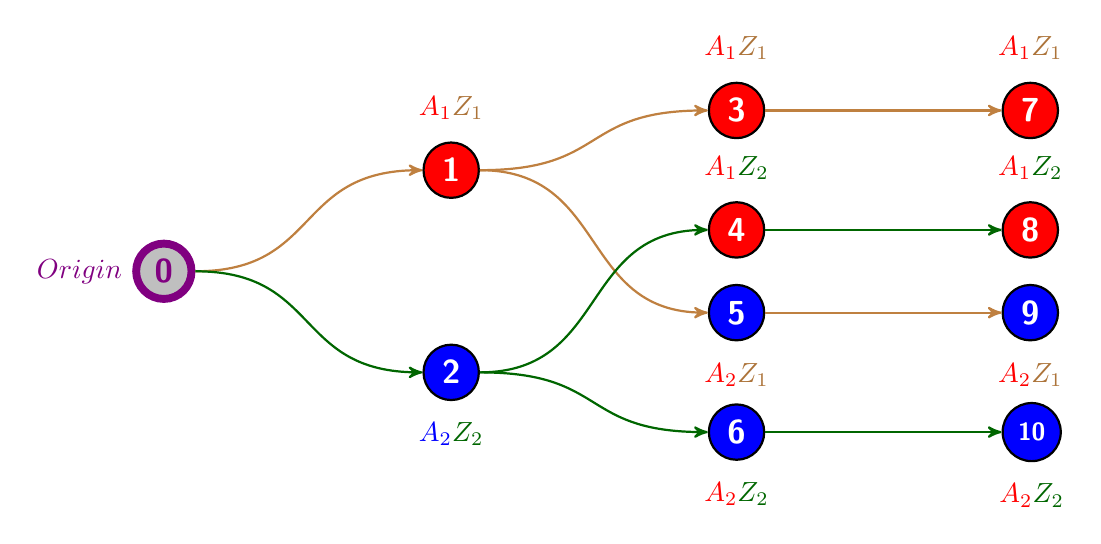
\begin{tikzpicture}[->,>=stealth',auto,node distance=7mm,
  thick,main node/.style={circle,draw,font=\sffamily\large\bfseries}]
  
  \node[main node,violet,line width=1mm,fill=lightgray,anchor=east] (o) {0};
    \node[left=0mm of o,anchor=east,violet] (x) {$Origin$};
  \node[main node,above right=1cm and 3cm of o,fill=red,anchor=west] (S1) {\color{white}1};
  \node[main node,below right=1cm and 3cm of o,fill=blue,anchor=west] (S2) {\color{white}2};
  \node[main node,above right=5mm and 3cm of S1,fill=red,anchor=west] (S3) {\color{white}3};
  \node[main node,below right=5mm and 3cm of S1,fill=red,anchor=west] (S4) {\color{white}4};
  \node[main node,above right=5mm and 3cm of S2,fill=blue,anchor=west] (S5) {\color{white}5};
  \node[main node,below right=5mm and 3cm of S2,fill=blue,anchor=west] (S6) {\color{white}6};
  \node[main node,right=3cm of S3,fill=red,anchor=west] (S7) {\color{white}7};
  \node[main node,right=3cm of S4,fill=red,anchor=west] (S8) {\color{white}8};
  \node[main node,right=3cm of S5,fill=blue,anchor=west] (S9) {\color{white}9};
  \node[main node,right=3cm of S6,fill=blue,anchor=west] (S10) {\color{white}\small 10};
  \node[above=of S1,anchor=north] {\color{red}$A_1\color{black!10!brown}Z_1$};
  \node[below=of S2,anchor=south] {\color{blue}$A_2\color{black!60!green}Z_2$};
  \node[above=of S3,anchor=north] {\color{red}$A_1\color{black!10!brown}Z_1$};
  \node[above=of S4,anchor=north] {\color{red}$A_1\color{black!60!green}Z_2$};
  \node[above=of S7,anchor=north] {\color{red}$A_1\color{black!10!brown}Z_1$};
  \node[above=of S8,anchor=north] {\color{red}$A_1\color{black!60!green}Z_2$};
  \node[below=of S5,anchor=south] {\color{red}$A_2\color{black!10!brown}Z_1$};
  \node[below=of S6,anchor=south] {\color{red}$A_2\color{black!60!green}Z_2$};
  \node[below=of S9,anchor=south] {\color{red}$A_2\color{black!10!brown}Z_1$};
  \node[below=of S10,anchor=south] {\color{red}$A_2\color{black!60!green}Z_2$};
  \draw[->,brown] (o) .. controls ([xshift=2cm] o) and ([xshift=-2cm] S1) .. (S1);
  \draw[->,brown] (S1) .. controls ([xshift=2cm] S1) and ([xshift=-2cm] S3) .. (S3);
  \draw[->,brown] (S1) .. controls ([xshift=2cm] S1) and ([xshift=-2cm] S5) .. (S5);
  \draw[->,black!60!green] (S2) .. controls ([xshift=2cm] S2) and ([xshift=-2cm] S4) .. (S4);
  \draw[->,black!60!green] (S2) .. controls ([xshift=2cm] S2) and ([xshift=-2cm] S6) .. (S6);
  \draw[->,black!60!green] (o) .. controls ([xshift=2cm] o) and ([xshift=-2cm] S2) .. (S2);
  \draw[->,brown] (S3) to (S7);
  \draw[->,brown] (S5) to (S9);
  \draw[->,black!60!green] (S4) to (S8);
  \draw[->,black!60!green] (S6) to (S10);
\end{tikzpicture}

\end{center}
\caption{Plasma assets flows are a simpler version of the classic UTXO model. }
\label{plasmautxomodel}
\end{figure}

Fig. \ref{plasmautxomodel} illustrates the coin flow when an Account $A_1$ deposits $Z_1$, an Account $A_2$ deposits $Z_2$ and they trade portions of the assets with each other.

The set of state changes has the signature of all parties plus the signature of the operator and is replicated among the network. The new states obsolete the old states, i.e., the balance at \(state_2: (A_1, Z_2) \) is spent/obsoleted by an updated balance at \(state_6: (A_1, Z_2)\). Further trades among the same assets update the existing balances to new states: if $A_2$ sells some more $Z_2$, $state_6$ will be updated to $state_{10}$. Additional non-obsoleted balance entries are created only when an account acquire an asset it did not previously own.

The validity of a balance entry can be verified by tracing the integrity and witness data all the way back to the origin just like an UTXO system. Such tracing is expensive and impractical for any high-volume system. We take the same approach as blockchain based coins and amortize the cost by validating changes in real-time. 

\subsection{Gluon Blocks}
State transitions are organized into blocks that are committed to the plasma contract called \emph{Gluon Blocks} or \emph{G-Blocks} at regular intervals called \emph{submissionInterval}. The commitment contains the following:

\begin{table}[ht]
\caption{Block Header committed to the main chain on the Gluon Plasma Smart Contract.}
\centering
\begin{tabular}{|l|l|}
\hline
\bfseries Field Name &\bfseries  Description \\
\hline
$gBlockNumber$ & G-Block number, increasing positive integer \\ 
$depositRoot$ & Ordered Merkle root of all valid deposits in this G-block \\ 
$withdrawRoot$ & Merkle root of all withdraw entries in this G-block \\ 
$balanceRoot$ & Merkle root of current balances snapshot as of this G-block\\ 

\hline
\end{tabular}
\end{table}

As users trade on the plasma sidechain, their balances change, and ledger entries are created to reflect every new balance. These balances are not yet in any G-Block and are considered to be in the \emph{Mempool}. These transactions are immediately eligible for fraud-proofs if the operator has shown fraudulent behavior. 

The operator accumulates entries from the \emph{Mempool} and periodically commits the most recent transactions to the plasma contract as a new G-block. The most recent G-block committed is said to be \emph{unconfirmed} and not usable for withdrawal, since the operator may have generated it by including invalid entries. A minimum challenge period needs to elapse to give participants a chance to verify the new G-block or submit a vote to halt the sidechain in case of data unavailability. Once the period has elapsed and a new \emph{unconfirmed} G-block has been committed, the prior G-block is deemed \emph{confirmed} and can be used for withdrawals. A user may also withdraw funds by showing proof of the exit claim by providing the Merkle proof of its entry in a confirmed G-block.

The root hashes above are also computed by network participants in real-time as new ledger entries are published. If the root hashes do not match the values committed to the plasma contract, there is a potential data unavailability issue and the participant can vote to halt. Naturally, participants should sync and obtain any missing entries if they have suffered from recent downtime or network disruption to avoid false signals.

\begin{table}[ht]
\caption{Ledger entries from \emph{Mempool} are committed to G-blocks periodically. The last G-block committed (G-block 3) is unconfirmed and unavailable for withdrawal.}
\centering
\begin{tabular}{|c|}
\hline
\rowcolor{green!50}G-Block 1 (confirmed) \\
\rowcolor{green!30}TX1 to TX 130 \\
\hline
\rowcolor{green!50}G-Block 2 (confirmed) \\
\rowcolor{green!30}TX131 to TX 526 \\
\hline
\rowcolor{orange!50}G-Block 3 (unconfirmed) \\
\rowcolor{orange!30}TX 527 to TX 785 \\
\hline
Mempool \\
TX 786 onwards \\
\hline
\end{tabular}
\end{table}

If proof of operator compromise is submitted to the plasma contract, then all transactions in the unconfirmed G-block and Mempool are effectively rolled back. This prevents a maleficent operator from withdrawing funds using fake balances.

\section{Characteristics of Gluon Plasma}
\subsection{Account Based}
Account based plasma can be seen as a structural constraint of having only one UTXO per asset per account called the \emph{balance}. 

When a recipient receives funds, the balance of that asset type is also spent, resulting in a new unspent balance output whose value is the sum of the spent balance and received funds.

This concept collapses the multi-branch UTXO graph into a single chain and allows us to reason about account safety in far simpler terms and create a comprehensive set of simple and compact fraud proofs. 

The external address that deposits the funds can be used as an account identifier enabling seamless enforcement of \emph{Segregation} and \emph{Agency} constraints. 

This approach also simplifies fraud proofs and orchestration of transactions:

\begin{enumerate}
    \item \emph{No UTXO Shredding.} Even with millions of matches, the user only has one balance per asset instead of the millions that would need to be managed in a pure UTXO system. 
    \item \emph{Predictable  Sidechain Characteristics.} For example, we can compute bounds for exiting to the main chain in case of a compromise, which is simply the product of the number of users and assets. 
    \item \emph{Compact Transactions.} Instead of picking the best set of UTXOs to fit the size of the trade and assemble them into acceptable transaction sizes, we simply have fixed size transactions. 
    \item \emph{Compact Proof-of-Ownership.} We do not require a chain of signatures from the creation of the UTXO into the plasma sidechain or periodic consolidations in the main chain to manage UTXO bloat. The latest balance is the single source of truth.
    \item \emph{Compact Fixed-Size Fraud-Proofs.} A later balance invalidates all prior balances. This enables compact, fixed-size fraud proofs that can be submitted to the plasma contract at predictable gas costs. 
\end{enumerate}

\subsection{Small Footprint}
One of the important distinctions of Gluon plasma versus other DEX is the small footprint in terms of state required on both the main chain and the plasma sidechain. The main chain footprint is limited to deposits, withdrawals and periodic commitments of the plasma sidechain. The commitments are a constant cost and do not change with trade volume or user activity. Deposits and withdrawals costs are similar to centralized exchanges. 
On the plasma sidechain, since every new balance invalidates the prior balance, validating nodes do not need to hold the the full sidechain history. 

\subsection{Instant Finality}
In coins with probabilistic finality (most POW and POS based coins) an observed transaction needs to be buried under work and/or time before it can be acted upon by an observer. For payment systems, a few seconds or even minutes may be acceptable for in-person transactions; much longer delays maybe acceptable for online transactions. In a trading application, finality must be instant, i.e., an observed transaction \emph{must} be accepted and actionable. This is because a filled transaction needs to trigger other actions, which when delayed can lead to losses. An example is setting stop orders when an entry order is filled or cancelling stop orders when a profit is taken. Having to wait even for a few seconds could mean the stop order cannot be set due to market movement.

Instant finality is accomplished by having the operator sign each execution with the exchange operator’s private key. This key should not have access to any funds. 

Instant finality also eliminates the “free option.” In systems where the two matched parties have to transmit the transaction to each other for mutual signatures, the trader who signs it last has a free option, where he can choose to sign only if the trade has moved in his favor. 

Having the operator match and countersign user-signed orders also eliminates the need to be online during a match. Participants can treat the exchange as a central counterparty and the fills are non-interactive once orders are placed. Natural trading behavior such as placing an order and closing the laptop computer is fully supported. Complex order types such as OTO/OCO orders\cite{invOT} are greatly simplified by making the order execution non-interactive.

While transfers within the sidechain have instant finality, transfers between main chain and sidechain have between 2 to 5 G-blocks to finality.

\subsection{Fast Withdrawal}
Having a POA system also enables fast withdrawals in the substantial portion of the time when the operator is behaving normally. Any faulty withdrawal can be immediately detected by any observer who can submit a fraud proof to the plasma contract.

\subsection{Compact Fraud-Proofs for Every Transition}
While POA is the direct route to instant finality, the authority of the exchange needs to be strictly limited to the authorized intentions of market participants according to the publicly agreed upon rules of the system. The exchange should not permit users to trade amounts in excess of their balance or create fake balances out of nothing. If a user authorizes buying \numprint{1000} tokens for 1 ether by signing the order with their private key, then the operator should only be able to fill the order within those parameters. 

Detection of any of these violations are simple, without undue burden of storage or computation on the part of the observer. We accomplish this by verifying the enforcement of all four trustless constraints for every state transition. On detecting any violations, the last valid state and the succeeding invalid state may be submitted to the plasma contract as a fraud-proof. The plasma contract halts the sidechain and enables all users to withdraw funds at leisure on submission of valid fraud-proofs.

Any aspect of the blockchain that can grow boundlessly with no or low cost will result in spam attacks and make verification onerous, causing only well-funded players to participate in the network. This includes proofs and therefore, proofs should be of constant size and easily computable. Fraud-proofs are of constant size when all information regarding correctness can be deduced from the combination of the prior state, change requests and the new state.

All validator proofs are non-interactive which makes operating a validator simple and cheap. 

\subsection{Non-onerous Safety}
The cost of ensuring safety of the network should be cheap in terms of both effort and resources. Some plasma variants require users to check the plasma sidechain every week or so to ensure their funds are not stolen. This implies that withdrawals to main chain would take about two weeks. In contrast, Bitcoin and other classic cryptocurrencies require no verification of the blockchain to ensure your funds are not stolen. Onerous safety is equivalent to cheap attacks and vice-versa. Safety should rest on a very few actors acting honestly. In Gluon plasma, only one validator needs to be honest and present to prevent a compromised operator from stealing funds. 

\subsection{Congestion Tolerant}
The protocol measures intervals in Gluon blocks where possible. This mitigates the effects of congestion on the main chain, enabling the plasma sidechain to continue operation mostly unaffected. Short downtimes can be accommodated without risk of protocol failure. 

\subsection{Incentive Balanced}
Incentive-balanced protocols where malicious actors have to expend resources and effort and normal users do not have to, are robust. The larger the incentive to cheat, the more expensive an action needs to be. In Gluon plasma, simple holding an asset is free.

\subsection{Chain Halt on Data Unavailability}
The plasma sidechain can also be halted in case of data unavailability. Block withholding is an attack by the operator where blocks are created but some or all ledger entries are not broadcast. Block withholding can be detected but not proven since there is insufficient data available for fraud proof submission. Block withholding attacks are handled by users exiting their funds from the main chain. 

\textbf{Voting.} This is accomplished by a threshold voting to halt the sidechain. To enable everyone to vote in a reasonable amount of time, the sidechain will be slowed based on the stake size that has chosen to vote. Since account sizes follow a power-law distribution and since the biggest accounts are likely to monitor the plasma sidechain, the very first or second large stake will push the next block by a few days giving others time to vote their stake. It takes just a few of the largest stakeholders to bring the sidechain to a halt.

\textbf{Abandonment.} If the operator stops creating blocks for a very long time, the chain is said to be \emph{abandoned}, and a public method can be invoked on the plasma contract to halt the chain, allowing everyone to transfer funds to the main chain.

\section{The Gluon Plasma Protocol}

The Gluon plasma protocol only cares about custody. It has the following elements:

\begin{enumerate}
    \item Deposit
    \item Reclaim Deposit
    \item Withdrawal
    \item Exit Asset Balance
    \item Gluon Block Submission
    \item Vote to Halt
    \item Halt Abandoned Chain
    \item Fraud Proofs
\end{enumerate}

All protocol steps have state transitions that the operator needs to incorporate into the ledger by creating a new entry. These ledger entries contain witness data and are signed by the \emph{Operator}. These can be checked by any \emph{Validator} and a non-interactive fraud proof may be submitted to the plasma contract if the witness data is invalid. 

Users are normally only concerned with \emph{Deposit} and \emph{Withdrawal} steps. They will \emph{Reclaim Deposit} and \emph{Exit Asset Balance} on halted chains.

\subsection{Deposit}\label{gp:deposit}
\begin{mdframed}
\begin{enumerate}
    \item Account $A$ transfers quantity $N$ of asset $Z$ to plasma contract $C$. 
    \item $C$ computes the designated G-block $G$ in which this deposit would be committed\footnote{The deposit visibility is on a future G-block $G = G_{i+k}$; $k \geq 3$ is necessary to ensure sufficient main chain confirmations before the deposit is visible on the plasma sidechain.} on the plasma sidechain.
    \item $C$ computes and stores hash $H$ of \((A, Z, N, G, nonce)\).
    \item Operator $X$ creates a ledger entry $D$ referencing $H$ and crediting $N$ amount of $Z$ to $A$. $A$ can trade once $D$ is published.
    \item Operator $X$ commits an ordered Merkle root $depositRoot$ of all deposits for G-block $G$. Any ignored deposits need to be reclaimed by the user.
\end{enumerate}
\end{mdframed}


\textbf{Remarks.} 
The operator creates \emph{Deposit} ledger entries for every deposit that it deems valid, signs them and publishes them on the plasma sidechain. These entries are committed to the main chain as $depositRoot$.

\subsection{Reclaim Deposit}\label{gp:reclaim}
Account $A$ can reclaim an operator uncommitted deposit once $G$ is confirmed.
\begin{mdframed}
\begin{enumerate}
    \item $A$ submits \((A, Z, N, G, nonce)\) with exclusion proof (\(H \notin depositRoot\)).
    \item $C$ computes hash $H$ of \((A, Z, N, G, nonce)\) and verifies that $H$ has not already been reclaimed and has been excluded from $depositRoot$ of $G$.
    \item $C$ marks $H$ as reclaimed and transfers quantity $N$ of asset $Z$ to account $A$.
\end{enumerate}
\end{mdframed}

\textbf{Remarks.}
While any account can transfer any asset to the plasma contract, the operator will only add entries to the ledger for supported assets. Any unsupported assets will be ignored by the operator and the user should \emph{Reclaim Deposit} to retrieve them. An unacknowledged deposit is normal and not a griefing attack. 

Ignoring unsupported tokens also eliminates some spam attacks. In addition, the operator may choose to ignore tiny deposits.

The ability to reclaim an unacknowledged deposit directly from the smart contract without requiring the co-operation of the operator is an essential requirement for non-custodial operation.

\subsection{Withdrawal}\label{gp:withdrawal}
\begin{mdframed}
\begin{enumerate}
    \item Account $A$ submits a signed withdrawal request for quantity $N$ of asset $Z$ to operator $X$ off-chain. 
    \item Operator $X$ creates a \emph{Withdraw} ledger entry $W$ that reflects the new reduced balance of \((A, Z)\) and publishes it. $A$ can withdraw once $W$ is in a confirmed G-block.
    \item $A$ submits $W$ with inclusion proof \((W \in withdrawRoot)\) to plasma contract $C$. 
    \item $C$ verifies $W$ is valid and has not been already processed. $C$ stores hash of $W$ to prevent duplicate withdrawals and sends $N$ quantity of $Z$ to $A$ on main chain.
    \item If $W$ is not published within a reasonable time (griefing attack by $X$), $A$ should cancel all open orders for $Z$ and proceed to \emph{Exit Asset Balance}.
\end{enumerate}
\end{mdframed}


\textbf{Remarks.}
In normal operation, the user can withdraw very fast with the co-operation of the operator. From the user’s perspective, a withdraw request is submitted and approved after a short period of time following which, the user can withdraw the funds. 

\subsection{Exit Asset Balance}\label{gp:exit}
\begin{mdframed}
\begin{enumerate}
    \item Account $A$ submits ledger entry $E$ for Asset $Z$ with inclusion proof (\(E \in balanceRoot\)) of the last confirmed G-block to plasma contract $C$. 
    \item $C$ registers the exit claim for $E$ in G-block $G_i$.
    \item Operator $X$ cancels all open orders\footnote{Operator detects claims by monitoring events on the plasma contract.} and prevents further activity for \((A, Z)\).
    \item After $k$ G-blocks\footnote{\(k \geq 3\) is an implementation-specific parameter ensuring all transactions currently in the Mempool at the point of the initial exit claim are in a G-block.}, $A$ submits proof  of unchanged balance in the unconfirmed G-block $G_{i+k}$. (\(e \in G.balanceRoot; e \in G_{i+k}.balanceRoot\)).
    \item $C$ transfers balance of $Z$ to $A$ on main chain and marks \((A,Z)\) as $Exited$ by storing \(ExitBlock(A, Z) = G_{i+k}\) thus preventing all further activity for \((A, Z)\).
\end{enumerate}
\end{mdframed}


\textbf{Remarks.}  Exiting an account’s asset balance is a permanent cessation of activity for the account/asset pair. Normally, this is only needed when the operator refuses to honor a fast withdrawal.  Assets may be transferred on a halted chain using only the final step.

\subsection{Gluon Block Submission}\label{gp:block}
\begin{mdframed}
\begin{enumerate}
    \item Operator $X$ sends new G-Block $G_{i+1}$ to plasma contract $C$.
    \item $C$ stores $G_{i+1}$:
    \begin{enumerate}
        \item Ensure $G_{i+1}$ is valid (expected G-block number).
        \item Ensure \(block.number \geq submissionBlock \).
        \item Store $G_{i+1}$.
        \item Mark $G_i$ as \emph{confirmed} and $G_{i+1}$ as \emph{unconfirmed}.
        \item Update \(submissionBlock = block.number + submissionInterval\)
        \item Update \(voteTally = 0\)
    \end{enumerate}
\end{enumerate}
\end{mdframed}

\textbf{Remarks.} The operator must include all ledger entries since the last G-block without any omissions or reordering. The plasma contract enforces a minimum  of $submissionInterval$ main chain blocks between two G-blocks. 

\subsection{Vote to Halt}\label{gp:vote2halt}
\begin{mdframed}
\begin{enumerate}
    \item Account $A$ votes to halt chain by invoking \(halt()\) on staking contract $S$.
    \item $S$ computes $voteSize$ and submits to $C$.
    \begin{enumerate}
        \item Let $voteSize$ = Tokens\footnote{Leverj uses LEV tokens for staking and governance.} staked by $A$
        \item Reduce $A$’s stake balance by \(votingCost = voteSize \times votePrice\)
        \item $S$ submits $votingCost$ to $C$.
    \end{enumerate}
    \item $C$ tallies votes and halts the plasma sidechain if threshold is met:
    \begin{enumerate}
        \item Update \(voteTally \mathrel{+}= voteSize\)
        \item Update \(submissionBlock = delayFunc(voteTally)\)
        \item Halt Chain if \(voteTally > haltThreshold\)
    \end{enumerate}
\end{enumerate}
\end{mdframed}

\textbf{Remarks.} Ledger entries and G-block commitments can be used as fraud-proofs to ensure chain fidelity. If the operator  withholds some or all entries from the committed block to prevent a fraud-proof submission, stake holders should vote to halt the chain.

A polynomial function $delayFunc$ ensures that when even a small size of the stake votes to halt, the next G-Block is delayed significantly, giving observers and large stakeholders sufficient opportunity to vote to cross the halting threshold. 

Votes are tallied in $voteTally$. The expected outcome is big stake holders such as market makers vote with minimal delay and reach the threshold quickly and halt the plasma sidechain.

The parameter $haltThreshold$ (10\% of total supply) should be large enough that a random account shouldn’t be able to halt at will and disrupt the smooth functioning of the plasma sidechain but small enough that halting is highly likely if the largest four or five non-team stakeholders vote.

The parameter $votePrice$ (around 10\%) determines the amount the halt invoker is willing to sacrifice to halt the sidechain. This should be low enough to be an acceptable alternative to a compromised operator but high enough to deter frivolous halts.

A speedy halt enables orderly exit and appropriate action to be taken, including deploying a new contract (in case of a bug) or a total new deployment (in case of a security breach). The ideal values for these parameters are best determined empirically with halting games with test users.

All voting schemes are tradeoffs and will never be perfect. Moving beyond voting into provable correctness that can be verified by the plasma contract itself is a research subject we are actively pursuing.

\subsection{Halt Abandoned Chain}\label{gp:abandon}
\begin{mdframed}
\begin{enumerate}
    \item Account $A$ calls $abandon$ on  plasma contract $C$
    \item $C$ halts chain if \(block.number > submissionBlock + abandonPoint\)
\end{enumerate}
\end{mdframed}

\textbf{Remarks.} The Gluon plasma system transitions among states on actions by the operator, validators or stakers voting to halt. This protocol step ensures that if all other actors  abandons the chain, a lone user can still transfer funds back to the main chain.

\subsection{Fraud Proofs}
The Gluon plasma smart contract is not aware of trades and real-time balances of any accounts but it does know about fraud proofs and how to enforce them. 

The operator facilitates trades between buyers and sellers who submit their signed orders. The signature from their private key is essential to prove that the trade is duly authorized and trade execution is within the parameters authorized by the participants.

A trade execution contains the fill parameters and include both buy and sell orders along with the operator’s countersignature. The operator signature prevents users from creating fills on their own and fabricating balances. 

The signatures and rules of the system are encoded as fraud proofs into the Gluon contract and security is predicated on having at least one honest validator able and willing to submit fraud proofs to the contract.

\subsection{General Protocol Characteristics}
\subsubsection{Spam Attacks}
Flooding the plasma sidechain with \emph{Deposit} and \emph{Exit} requests is an unlikely attack vector, since the gas cost alone should be a discouragement for this attack. The net impact of a spam attack is reduced on-chain bandwidth for deposits and withdrawals.

Voting to halt costs a significant amount of governance tokens and should discourage careless voting or deliberate griefing.

\subsubsection{Network Congestion/Server Temporarily Offline }
If the operator is offline for a short duration of time (for maintenance or network/data center outage), balance updates, deposits and withdrawals can continue on the main chain but the corresponding ledger entries will be postponed until the operator comes back online.

\subsubsection{Contract Upgrade}
The operator halts all activity and submits a G-Block containing the final transactions. After the mandatory block submission delay, an empty G-block is also committed, thereby confirming the prior G-block. It then moves the plasma contract to a halted state. Users can use the \emph{Asset Balance Exit} protocol to extract and move funds to the upgraded contract.

\subsubsection{Halted State}
The operator determines the cause of the halt and takes any necessary corrective action and starts a new sidechain. The old chain is abandoned and users move their funds to the new chain. 

\section{Gluon Plasma Fraud Proofs}

We present a comprehensive suite of fraud proofs that address every possible state change. Fraud proofs are stated as assertions that need to be always true. Any failed assertion should halt the plasma sidechain. 

Voting to halt works as a catch-all fraud in case a new fraud that can be detected by not proven is found after the contract is live.

All fraud-proofs that require any operator signed ledger entry $e$ require verification of the operator signature to ensure authenticity.

\begin{equation}
    ecrecover(e) = operator
\end{equation}

\subsection{Gluon Protocol Frauds}

\subsubsection{Block Commitment Frauds.}\label{fp:bcf}
Data unavailability is detected as a mismatch between the observed ledger entries and their commitment. Every validator should compute commitment roots as they are published and if the commitment does not match the computed root, proceed to \emph{Vote to Halt}.

\textbf{Deposit Commitment Mismatch.} Operator commits deposit in $depositRoot$ but does not create a corresponding \emph{Deposit} ledger entry.

\textbf{Detection.} 
Committed $depositRoot$ does not match deposit commitment $M_D$ computed by plasma participants using published Gluon plasma \emph{Deposit} ledger entries for a given G-block, resulting in \emph{Vote to Halt}.

\begin{equation}
M_D = G.depositRoot
\end{equation}

\textbf{Withdraw Commitment Mismatch.} 
Operator commits a withdrawal in $withdrawRoot$ but does not create a corresponding \emph{Withdraw} ledger entry.

\textbf{Detection.} 
Committed $withdrawRoot$ does not match withdraw commitment $M_W$ computed by plasma participants using published Gluon plasma \emph{Withdraw} ledger entries for a given G-block, resulting in \emph{Vote to Halt}.

\begin{equation}
M_W = G.withdrawRoot
\end{equation}

\textbf{Balances Commitment Mismatch.} Operator creates a fake ledger entry in order to steal funds and commits in $balanceRoot$ but does not publish it to avoid detection.

\textbf{Detection.} Committed $balanceRoot$ does not match commitment $M_B$ computed for current snapshot as of a given G-block by plasma participants using all published Gluon plasma ledger entries, resulting in \emph{Vote to Halt}.

\begin{equation}
M_B = G.balanceRoot
\end{equation}

\subsubsection{Invalid Deposit Fraud}\label{fp:idf}
Operator creates a deposit entry with a fake, incorrect or already reclaimed deposit hash $H$ (i.e., credits an incorrect account, amount or asset) 

\textbf{Proof.} 
Operator signed \emph{Deposit} ledger entry $e$. The plasma contract $C$ cross-checks the entry hash as its own creation. An invalid deposit entry causes a chain halt.

    \[ H = hash(e.account, e.asset, e.quantity, e.gBlock, e.nonce) \]
    \begin{equation}
    C.deposits[H] = true
    \end{equation}


\subsubsection{Deposit Reversal Fraud}\label{fp:drf}
Operator does not include the deposit ledger entry $e$ in $depositRoot$ enabling user to reclaim the deposit and trade without funds. 

\textbf{Proof.} The deposit ledger entry $e$. Proof of exclusion of the deposit hash H of $e$ can be used as proof. As a practical matter, since the committed $depositRoot$ won't match the validator computed value, this will result in a \emph{Vote to Halt}.

\begin{equation}
    e.H \in G.depositRoot
\end{equation}

\subsubsection{Fake Withdraw Entry} \label{fp:fwe}
Operator creates an unauthorized or fake \emph{Withdraw} entry. The operator cannot steal these funds but can grief a user and prevent them from trading. 

\textbf{Proof.} Operator signed fake \emph{Withdraw} entry $e$. The plasma contract checks that the user signature does not match contents and chain is halted.
\begin{equation}
ecrecover(e.accountsignature) = account
\end{equation}


\subsubsection{Exit Insolvency Fraud}\label{fp:eif}
Exchange does not cancel \emph{Exited} orders, enabling trading without funds.

\textbf{Proof.} Insolvent ledger entry $e$ and Merkle proof in a post exit G-block. Existence of any ledger entry $e$ after \emph{Exited} balance is evidence of a compromised operator. To prevent loss, this proof must be submitted when the entry is still in an unconfirmed G-block $G_{i+1}$.
\begin{equation}
\exists ExitBlock(A,Z) = G_x \wedge e \in G_{i}.balanceRoot \implies i < x
\end{equation}

\subsubsection{Fake Exit Fraud}\label{fp:fef}
Operator creates a fake \emph{Exited} entry to grief the user.

\textbf{Proof.} Operator signed Exited entry $e$. An exit (A,Z) is saved in the plasma contract and can be easily checked.
\begin{equation}
    e.type=Exited \implies \exists ExitBlock(A,Z)
\end{equation}

\subsection{Ledger Entry Frauds}
\subsubsection{Fake Signature Fraud} \label{fp:fsf}
A maleficent operator can perform a skimming attack by creating fake orders of victim accounts. The operator may sign an account order with a fake API key\cite{levzkapi}. These orders may be used to pump prices or other forms of market manipulation.

\textbf{Proof} 
Any ledger entry $e$. An API key $originator$ for any account is verifiable by the plasma contract from API Key registry $R$. The fake order in the ledger entry would not have a valid signature of the account. To ensure that ledger entries are not created by a validator to fraudulently halt the chain, we have to also ensure that the ledger entry has been signed by the Operator.

\begin{equation}ecrecover(e.buyorder) = e.buyorder.account\end{equation}
\begin{equation}
ecrecover(e.sellorder) = e.sellorder.account
\end{equation}
\begin{equation}
    R.translate(e.buyorder.originator) = e.buyorder.account
\end{equation}
\begin{equation}
    R.translate(e.sellorder.originator) = e.sellorder.account    
\end{equation}
 
\subsubsection{FEE Fraud} \label{fp:fee}
The operator may give an excess fee to itself say, 100\% and steal everyone’s funds. The operator may also extract fees from an unauthorized asset or send the fee to an unauthorized recipient.

\textbf{Proof.} 
Any ledger entry $e$. The maximum fees ($MAX\_FEE$) that can be charged is enforced by the contract.
\begin{equation}
    e.type = FEE \implies e.fill.quantity \times MAX\_FEE \leq e.quantity
\end{equation}
\begin{equation}
    e.type = FEE \implies e.account = STAKING\_ADDR
\end{equation}
\begin{equation}
    e.type = FEE \implies e.asset \in FEE\_TOKENS 
\end{equation}

\subsubsection{Price Fraud} \label{fp:prc}
The operator may match victim orders at unfavorable prices and give its own orders a better price, enabling skimming.

\textbf{Proof.} Any ledger entry e that matched a limit order. Executions should fill at limit price or better . 

\begin{equation}
    e.fill.price \leq e.buyorder.price
\end{equation}
\begin{equation}
    e.fill.price \geq e.sellorder.price
\end{equation}


\subsection{Ledger Entry Ordering Frauds}
\subsubsection{Broken Chain Fraud}\label{fp:bc}
This is a data unavailability attack where the operator creates an entry with a non-existent prior entry.

\textbf{Proof.} There is no fraud-proof for this attack and would be handled by \emph{Vote to Halt}.
\subsubsection{Double-Spend Fraud}\label{fp:dsf}
The operator creates a ledger entry linking to a spent/obsolete ledger entry, i.e., two ledger entries have the same parent. As a practical matter, this fraud will be detected exactly as the \emph{Broken Chain Fraud} and will result in a chain halt.

\textbf{Proof.} Ledger entries $e_1$ and $e_2$ with same parent $p$ (other than \emph{Origin}).
\begin{equation}
    e_1.parent = e_2.parent \implies parent = \emph{Origin}
\end{equation}
\subsubsection{Counterfeit Fraud} \label{fp:cff}
When the ledger entries for a match are created, the operator may switch asset or accounts in ledger entry chain, inflate the balance of one of the accounts in a counterfeiting effort. Conversely, values may be fraudulently decreased for victims.

\textbf{Proof.} 
Most recent entry $e$ and prior entry $p$ for account $A$. Balances should add up to quantities transacted; asset and account provenance should hold.
\begin{equation}e.balance \geq 0\end{equation}
\begin{equation}
  e.balance = p.balance \pm e.quantity  
\end{equation}
\begin{equation}p.asset = e.asset\end{equation}
\begin{equation}p.account = e.account\end{equation}
\begin{equation}e.previous = p\end{equation}
\begin{equation}
entry.buyorder.asset = entry.sellorder.asset = entry.fill.asset
\end{equation}
\subsubsection{Replay/Overfill Fraud} \label{fp:rof}
The operator may match the same order multiple times or match it to higher than specified quantity.

\textbf{Proof.} 
Most recent execution entry $e$ and prior entry $p$ for order $o$. The chain of ledger entries from multiple fills would need to have incorrect fill quantities to perform this fraud. We can ensure the numbers add up and no orders have been replayed or overfilled.
\begin{equation}p.o.filled + e.fill.quantity = e.o.filled\end{equation}
\begin{equation}
    e.o.filled \leq e.o.quantity
\end{equation}
\subsubsection{Price Time Priority Fraud}\label{fp:ptp}
This is a versatile fraud proof that can detect a variety of exchange frauds. In particular, it can detect front running, holding orders hostage for skimming and in general, all frauds where the exchange is required to violate the predefined Central Limit Order Book (CLOB) behavior. 

The proof is based on the fact that front-running and other skimming frauds are a form of illegal arbitrage that use advance knowledge of order flow. Profitable arbitrage is only possible when the operator can exit at a profitable price differential. Anything else is economically identical to a normal legal entry.

\textbf{Market Orders.} A victim order sufficiently large to move the price can be front-run. For example, if the bid/ask is 50@2.00/80@3.00, and if the victim places a buy market order for quantity of 100, the frontrunner would insert a buy order to take the existing 80 asks at 3.00 and place a take profit sell order just before the next order in line to be filled. Frontrunning on market orders are undetectable since market orders have the highest priority.

\textbf{Limit Orders.} Limit orders cannot be front-run as above since any unfilled quantity turns into a resting order. When filling deep into the orderbook, a fill-or-kill flag would ensure that the trader will not pay more than he expects.

To front-run limit orders, the frontrunner would have to hold on to the victim order and wait for the price to move against the victim and then fill both the victim order and a take profit order near simultaneously. This is observed as an order that filled out of turn, i.e., an order with an earlier entry time was filled at a worse price. 

\textbf{Proof.} Recent entry $e$ and prior entry $p$ for the same asset and market side.

\begin{equation}
e.order.price \succcurlyeq p.order.price\footnote{We use the symbol $\succcurlyeq$ to denote same or worse price (higher buys and lower sells.)} \implies e.order.created > p.filltime    
\end{equation}

For price-time priority fraud to work correctly, it is necessary to ensure that the exchange does not accept orders with a clock that is far beyond the skew tolerance that would weaken the price-time priority fraud.

\textbf{Proof.} 
Any ledger entry $e$. The execution of orders should not precede the orders and the clock skew between the user’s clock and the operator’s clock must be within the system tolerance $MAX\_SKEW$.
\begin{equation}e.buyorder.exchangeTime \leq e.fill.exchangeTime\end{equation}
\begin{equation}e.sellorder.exchangeTime \leq e.fill.exchangeTime\end{equation}
\begin{equation}\mid e.order.originatorTime - e.order.exchangeTime \mid < MAX\_SKEW\end{equation}
\subsubsection{Unit Fraud}\label{fp:uf}
Every ledger entry represents an entire state change. The exception is an execution, which is represented by four \emph{Trade} entries and up to four \emph{Fee} entries. The operator may put fewer or more entries to violate solvency.

\textbf{Proof.} \emph{Trade} entries for a given execution $ex$ should have exactly four entries and their quantities should add up to zero. Similarly, two or four \emph{Fee} entries $f_i$ may exist per execution. If not, validators proceed to \emph{Vote to halt}.
\begin{equation}
    ex.length = 4
\end{equation}
\begin{equation}
ex(A_1,Z_1).Qty = -ex(A_2,Z_1).Qty
\end{equation}
\begin{equation}
ex(A_2,Z_2).Qty = -ex(A_1,Z_2).Qty 
\end{equation}


\begin{equation}
    fee.length = 4 \lor fee.length = 2
\end{equation}
\begin{equation}
fee(A_1,Z_1).Qty = -fee(A_2,Z_1).Qty 
\end{equation}
\begin{equation}
fee(A_2,Z_2).Qty = -fee(A_1,Z_2).Qty 
\end{equation}
\subsection{Validator Considerations}

\subsubsection{Storage} 
Most fraud proofs require only the most recent entry, which contains sufficient information to prove its validity. These can be statelessly validated. 

Solvency proofs require keeping track of the last balance of every asset for every user. When a new balance entry is observed, the new and old entries can be used to verify validity of the transaction. An invalid change results in a fraud proof submission and a valid entry results in the new entry replacing the old. The storage requirement would be: \emph{number of minimum-balance accounts $\times$ number of listed assets}.

Overfill and price-time priority proofs requires retaining references to the last \emph{Trade} and \emph{Fee} ledger entries of every Asset regardless of user. The maximum space required is: \emph{2 $\times$ number of listed assets}.

\subsubsection{Adverserial} Spam attacks to overwhelm validators would require an attacker to create an excessive number of accounts since listing assets is controlled by the exchange. Requiring a minimum balance to trade, minimum withdrawal sizes and a reasonable tick size should ensure that validators are not spammed by millions of dust accounts. 

\section*{Future Work}
Zk-snarks or zk-starks may be a succinct alternative to a large set of separate proofs. A complete chain of proof-of-correctness exist between main-chain commitments. If these can be coalesced into a single compact proof that can be committed to the main-chain and verified by the plasma contract, the data unavailability problem can be eliminated, enabling us to eliminate unconfirmed blocks and voting to halt. This is an active research subject at the time of this writing.

The same plasma chain can support multiple operators who need to coordinate the plasma operations. These exchanges are incentivized by revenue sharing to share their unfilled orders with peer exchanges. Consequently, deposits and trades on the plasma chain will appear on all exchanges, mitigating the effects of downtime of a single exchange.

\section*{Acknowledgment}
Gluon plasma is a product of teamwork and the protocol would not be possible without the extensive efforts of the full leverj.io team. In particular, N. Gupta for fixing many security issues and making the protocol robust with great attention to detail, B. Sadeh for simplifying deposits and ensuring the protocol remains simple, S. Tiwari for help with proofs and C. Engel for critical input from product fit and market perspective.

\begin{thebibliography}{999}
\bibitem{Nak09}
S. Nakamoto. Bitcoin: A Peer-to-Peer Electronic Cash System. \\
\url{https://bitcoin.org/bitcoin.pdf}, 2009.

\bibitem{Eth14}
Ethereum. A Next-Generation Smart Contract and Decentralized Application Platform. \\
\url{https://github.com/ethereum/wiki/wiki/White-Paper}, 2013.

\bibitem{Gav15}
G. Wood. Ethereum: A Secure Decentralized Generalized Transaction Ledger.
\url{https://gavwood.com/paper.pdf}, 2014.

\bibitem{PB17}
J. Poon, V. Buterin. Plasma: Scalable Autonomous Smart Contracts\\
\url{http://plasma.io/plasma.pdf}, 2017.

\bibitem{nakcons}
N. Stifter, A Judmayer, P Schindler, A Zamyatin, E Weippl. Agreement with Satoshi – On the Formalization of Nakamoto Consensus\\
\url{https://eprint.iacr.org/2018/400.pdf}, 2018.

\bibitem{DN93}
C. Dwork, M. Naor. Pricing via Processing or Combatting Junk Mail.\\ \url{http://www.hashcash.org/papers/pvp.pdf}, 1993.

\bibitem{parPOA}
parity.io \url{https://wiki.parity.io/Proof-of-Authority-Chains}.

\bibitem{Max13}
G. Maxwell. CoinJoin. \url{https://bitcointalk.org/?topic=279249}, 2013.

\bibitem{BTCProtocol}
Bitcoin.it \url{https://en.bitcoin.it/wiki/Protocol_documentation}.

\bibitem{BTCColdStorage}
Bitcoin.it \url{https://en.bitcoin.it/wiki/Cold_storage}.

\bibitem{DLRS14}
A. Dmitrienko, C. Liebchen, C. Rossow, A. Sadeghi. Security Analysis of Mobile Two-Factor Authentication Schemes. \\
\url{http://www.icri-sc.org/fileadmin/user_upload/Group_TRUST/PubsPDF/Dmitrienko-127-camera-ready.pdf}, 2014.

\bibitem{levprotocol}
B. Rao, N. Gupta. Leverj Decentralized Custody. \\
\url{https://leverj.io/LeverjProtocol.pdf}, 2017.

\bibitem{WA17}
W. Warren, A. Bandeali. \\
\url{https://0xproject.com/pdfs/0x_white_paper.pdf}, 2017.

\bibitem{invOT}
investopedia.com \url{https://www.investopedia.com/terms/o/oco.asp}.

\bibitem{levzkapi}
N. Gupta. Zero Knowledge API Keys. \\ \url{https://blog.leverj.io/zero-knowledge-api-keys-43280cc93647}, 2018.
\end{thebibliography}
\ClearShipoutPictureBG

\appendix
\newpage
\section{Safety of Trustless Constraints}\label{app:safety}
\begin{figure}[h]
\centering

\subfloat[][Banking]{
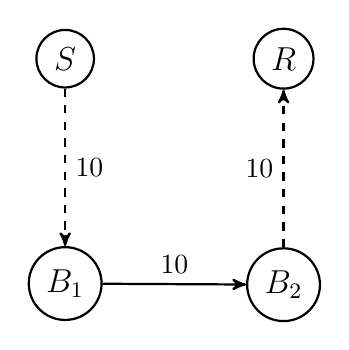
\begin{tikzpicture}[->,>=stealth',auto,node distance=2,
  thick,main node/.style={circle,draw,font=\sffamily\large\bfseries}]
    \node[main node](A1){$S$};
    \node[main node,below=of A1](C1){$B_1$};
    \node[main node,right=of A1](A2){$R$};
    \node[main node,below=of A2](C2){$B_2$};
    \path[dashed] (A1) edge node {10} (C1)
                  (C2) edge node {10} (A2)
    ;
    \path 
          (C1)  edge node {10} (C2)
    ;
\end{tikzpicture}
}
\qquad
\qquad
\subfloat[][Credit Cards] {
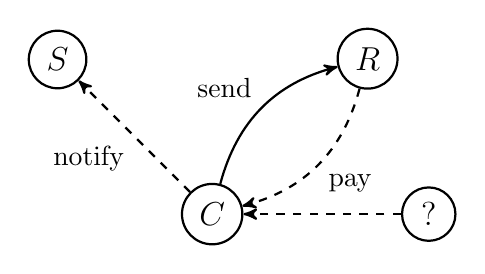
\begin{tikzpicture}[->,>=stealth',auto,node distance=2,
  thick,main node/.style={circle,draw,font=\sffamily\large\bfseries}]
    \node[main node](A1){$S$};
    \node[main node,below right=of A1](C){$C$};
    \node[main node,above right=of C](A2){$R$};
    \node[main node,right=of C](Q){$?$};
    \path[dashed,bend left] (A2) edge node {pay} (C);
    \path[dashed] (Q) edge node {} (C);
    \path[dashed]           (C) edge node {notify} (A1);
    \path[bend left] (C) edge node {send} (A2);
\end{tikzpicture}
}

\subfloat[][Postal]{
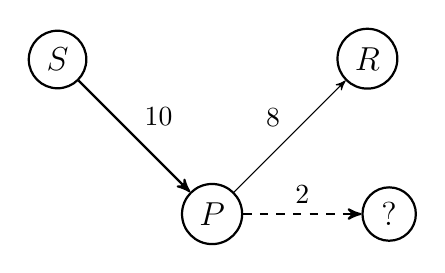
\begin{tikzpicture}[->,>=stealth',auto,node distance=2,
  thick,main node/.style={circle,draw,font=\sffamily\large\bfseries}]
    \node[main node](A1){$S$};
    \node[main node,below right=of A1](C){$P$};
    \node[main node,above right=of C](A2){$R$};
    \node[main node,right=1.5 of C](Q){$?$};
    \path (A1) edge node {10} (C);
    \path (C)[thin]  edge node {8} (A2)
    ;
    
    \path[dashed] (C) edge node {2} (Q)
    ;
\end{tikzpicture}
}
\qquad
\qquad
\subfloat[][Hawala]{

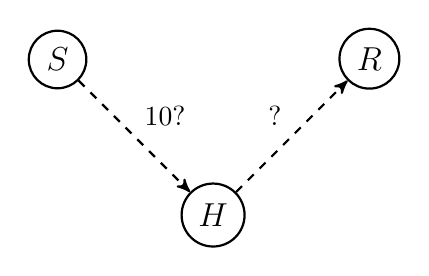
\begin{tikzpicture}[->,>=stealth',auto,node distance=2,
  thick,main node/.style={circle,draw,font=\sffamily\large\bfseries}]
    \node[main node](A1){$S$};
    \node[main node,below right=of A1] (H) {$H$};
    \node[main node,above right=of H](A2){$R$};
    \path[dashed] (A1) edge node {10?} (H)
          (H)  edge node {?} (A2)
    ;
    
\end{tikzpicture}
}

\subfloat[][Crypto]{

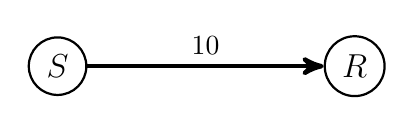
\begin{tikzpicture}[->,>=stealth',auto,node distance=3,
  thick,main node/.style={circle,draw,font=\sffamily\large\bfseries}]
    \node[main node](A1){$S$};
    \node[main node,right=of A1](A2){$R$};
    \path[ultra thick] (A1) edge node {10} (A2)
    ;
\end{tikzpicture}
}


\caption{Custodial characteristics of payment networks.}
\label{fig:custody}
\end{figure}

\textbf{Banking.} Payments are settled between member banks. The recipient waits for the bank to processes the transaction, deduct fees and release a portion for withdrawal. No \emph{Segregation} implies risk of censorship and seizure.

\textbf{Credit Cards.} Anyone with the card information can initiate a payment. Elaborate fraud detection schemes are needed to compensate for the lack of \emph{Agency} in the system design.

\textbf{Postal Service.} Some packages sent through the mail may be irreplacably lost. Even when using registered mail, there is no way to guarantee that all items sent will be received. The system lacks \emph{Solvency} and is not usable for items of high value.

\textbf{Hawala.} The rest of the Hawala network cannot verify that a payment has indeed been correctly made. No \emph{Integrity} enforcement inhibits the Hawala network growth beyond trusted family and kin. 

\textbf{Crypto.} Crypto networks require a signature from the sender's private key. The payment is sent directly into the recipients public key. Network participants can observe the signature and validate the exact payment amount and update their ledgers. This network enforces all four constraints.

\newtheorem{theorem}{Theorem}
\begin{theorem}
Provably safe payments between participants in a payment network is only possible when all intermediaries are perfectly safe.
\begin{proof}
Let the digraph $G=(V,E)$ represent a payment network where $V$ is the set of members and $E$ is the set of interconnections. Let $\Pi_s$ represent the set of all paths beginning with $v_s$. Let $\Pi^t$ represent the set of all paths ending at $v_t$. 

The set of all payment routes between $v_s$ and $v_t$ that $v_s$ can use to send a payment to $v_t$ is

\begin{equation}
  \Pi_s^t = \Pi_s \cap \Pi^t  
\end{equation}

Let $P_i$ be the probability of loss of safety during payment forwarding at each node $v_i$ of any path $\Pi_i$ in $\Pi_s^t$.
The cumulative probability $P$ of loss of safety at least a single node along $\Pi_i$ is 
\begin{equation}
    P = \sum_0^n P_i 
\end{equation}
\begin{equation}
    P = 0 \iff n = 0 \lor \forall i, P_i = 0
\label{T1eq1}
\end{equation}

Loss of safety is zero if and only if there are perfect or no intermediaries.
\end{proof}
\end{theorem}
\newtheorem*{remark}{Remark}
\begin{remark}{} The outgoing edge from $v_s$ represents \emph{Agency}. The incoming path to $v_t$ represents \emph{Segregation}. Having only perfect or zero intermediaries represents \emph{Solvency}. The ability of other participants to verify the existence of the edge $(v_s,v_t)$ represents \emph{Integrity}.
\end{remark}
\newtheorem{corollary}{Corollary}
\begin{corollary}
A series of perfect intermediaries between two network participants is equivalent to having no intermediaries.
\begin{proof}
A perfect intermediary is transitive. 
\begin{equation}
    v_s \rightarrow v_i \rightarrow v_t \implies v_s \rightarrow v_t
\end{equation}
Perfect intermedairy nodes can be disregarded from analysis and a series of perfect intermediaries from vertex $v_s$ to $v_t$ is equivalent to a   directed edge from $v_s$ to $v_t$. 
\end{proof}
\end{corollary}
\begin{remark}
A path consisting of a single directed edge or equivalent from the sender to  receiver represents the four trustless constraints. 
\end{remark}
\newpage
\section{Proof of Custody}
\begin{figure}[ht]
    \centering
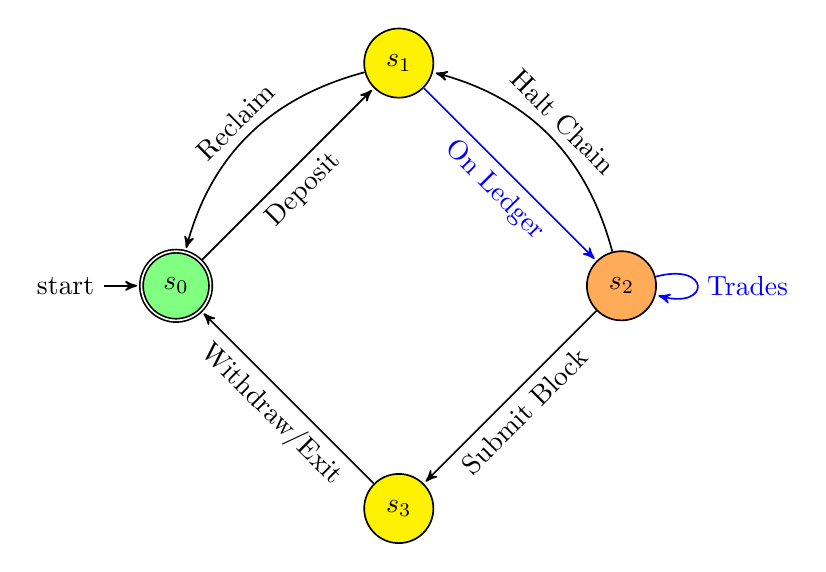
\begin{tikzpicture}[->,>=stealth',shorten >=1pt,auto,node distance=4cm,
                    semithick]
%  \tikzstyle{every state}=[fill=red,draw=none,text=white]

  \node[initial,state,accepting,fill=green!50] (A)                    {$s_0$};
  \node[state,fill=yellow]         (B) [above right of=A] {$s_1$};
  \node[state,fill=yellow]         (D) [below right of=A] {$s_3$};
  \node[state,fill=orange!66]         (C) [below right of=B] {$s_2$};
 
  \path[every node/.style={sloped,anchor=north,auto=false}]
        (A) edge   node {Deposit} (B)
        (B) edge [bend right] node [anchor=south,auto=true] {Reclaim} (A)
            edge [color=blue]  node {On Ledger} (C)
        (C) edge [bend right]  node [anchor=south,auto=true] {Halt Chain} (B)
            edge [color=blue,loop right,anchor=east,auto=true] node [sloped=false,anchor=west,auto=true] {Trades} (C)
            edge              node {Submit Block} (D)
        (D) edge              node {Withdraw/Exit} (A);
 \end{tikzpicture}

    \caption{State Diagram of user funds custody}
    \label{fig:custodystate}
\end{figure}

In Fig. \ref{fig:custodystate}, State $s_0$ represents funds on the main chain under direct control of the user's private key. States $s_1$ and $s_3$ represent funds on the plasma contract that the user can move back to $s_0$ without the need for any other parties. State $s_2$ represents uncommitted balance changes in the plasma chain. We prove continuous user custody by showing that the user can always move funds to $s_0$. 

The user initiates a deposit into the plasma chain using the \emph{Deposit} step of the protocol, moving funds from $s_0$ to $s_1$. State $s_1$ represents funds deposited by the user into the Plasma smart contract waiting to be credited into the plasma chain by the operator. Funds on state $s_1$ will move to state $s_2$ after $k$ blocks. If not, the user can move funds back to $s_0$ using the \emph{Reclaim Deposit} step.

State $s_3$ represents committed balances on a confirmed plasma block. Confirmed changes can be moved to $s_0$ using the \emph{Withdrawal} or \emph{Exit Asset Balance} protocol steps.

State $s_2$ represents funds on the actual plasma chain in unconfirmed blocks or the \emph{Mempool}. During normal operation of the chain, balance changes are periodically committed to the plasma contract and the funds move to state $s_3$ from where they can be moved as above. When the operator is compromised, the chain can be halted and state $s_2$ is effectively deleted. User funds remain in either $s_1$ or $s_3$ and can be directly moved to $s_0$. 


\newpage
\section{Gluon Plasma Proof of Safety}

The plasma system is safe only if every state change is safe. Enforcing the trustless constraints at every step of the protocol, every ledger entry and all ledger entry ordering creates a secure system. The tables below show all possible state changes and their enforcing fraud-proof or protocol step.

\begin{table}[ht]
\caption{\textbf{Gluon Plasma Protocol.} Every protocol step enforces all constraints.}
\centering
\begin{tabular}{|c|>{\columncolor{green!50}}c|>{\columncolor{violet!20}}c|>{\columncolor{yellow!50}}c|>{\columncolor{blue!20}}c|}
\hline
        \bfseries Step &\bfseries Segregation & \bfseries Agency & \bfseries Solvency & \bfseries Integrity \\
\hline
    Deposit & \ref{fp:idf} & \ref{fp:idf} & \ref{fp:idf} & \ref{fp:idf} \\
    Reclaim Deposit & \ref{gp:reclaim} & \ref{gp:reclaim} & \ref{gp:reclaim} & \ref{gp:reclaim} \\
    Withdraw & \ref{gp:withdrawal} & \ref{fp:fwe} & \ref{fp:cff} & \ref{fp:cff} \\
    Exit &	\ref{gp:exit} & \ref{fp:fef} & \ref{fp:eif} & \ref{fp:cff} \\
    Submit Block  &   \ref{fp:bcf}, \ref{fp:drf} &   \ref{fp:bcf} &   \ref{fp:bcf} &   \ref{fp:bcf} \\
\hline
\end{tabular}
\end{table}

\begin{table}[ht]
\caption{\textbf{Plasma Ledger Entries.} Every ledger entry enforces all constraints}
\centering
\begin{tabular}{|c|c|c|c|c|c|}
\hline
        \bfseries Field &\bfseries Deposit & \bfseries Withdraw & \bfseries Exit & \bfseries Trade & \bfseries Fee \\
\hline
    \rowcolor{yellow!50} Id & \ref{fp:bc}  & \ref{fp:bc}  & \ref{fp:bc}  & \ref{fp:bc}  & \ref{fp:bc} \\
    \rowcolor{yellow!50} Prior & \ref{fp:dsf}  & \ref{fp:dsf}  & \ref{fp:dsf}  & \ref{fp:dsf}  & \ref{fp:dsf} \\
    \rowcolor{yellow!50} Account &\ref{fp:idf}, \ref{fp:cff} & \ref{fp:cff} & \ref{fp:cff} & \ref{fp:cff} & \ref{fp:cff}\\
    \rowcolor{yellow!50} Asset & \ref{fp:idf}, \ref{fp:cff} & \ref{fp:cff} & \ref{fp:cff} & \ref{fp:cff} & \ref{fp:fee}\\
    \rowcolor{yellow!50} Balance  & \ref{fp:cff} & \ref{fp:cff} & \ref{fp:cff} & \ref{fp:cff} & \ref{fp:cff}\\
    \rowcolor{blue!20} Price & $-$ & $-$ & $-$ & \ref{fp:prc} & \ref{fp:fee}\\
    \rowcolor{blue!20} Qty & \ref{fp:idf}, \ref{fp:cff} & \ref{fp:cff} & \ref{fp:cff} & \ref{fp:cff}, \ref{fp:rof} & \ref{fp:cff}, \ref{fp:rof}\\
    \rowcolor{blue!20} Time & $-$ & $-$ & $-$ & \ref{fp:ptp} & \ref{fp:ptp} \\
    \rowcolor{violet!20} Witness & \ref{fp:idf} & \ref{fp:fwe} & \ref{fp:fef} & \ref{fp:fsf} & \ref{fp:fsf}\\
    \rowcolor{green!50} Segregation & \ref{fp:idf}	& \ref{gp:withdrawal} & \ref{gp:exit} & \ref{fp:fsf} & \ref{fp:fee}\\
\hline
\end{tabular}
\end{table}

\begin{table}[ht]
\caption{\textbf{Order of Ledger Entries.} Combinatorial attacks prevented.}
\centering
\begin{tabular}{|c|c|c|c|c|c|}
\hline
        \bfseries Attack &\bfseries Deposit  & \bfseries Withdraw & \bfseries Exit & \bfseries Trade & \bfseries Fee \\
\hline

\rowcolor{yellow!50} Unitary  & $-$  & $-$  & $-$  & \ref{fp:uf}  & \ref{fp:uf} \\
\rowcolor{yellow!50} Replay  & \ref{fp:bcf}  & \ref{gp:withdrawal} & \ref{fp:eif}   & \ref{fp:rof}, \ref{fp:ptp}  & \ref{fp:rof}, \ref{fp:ptp} \\
\rowcolor{yellow!50} Suppress  &   \ref{fp:bcf}  & \ref{gp:exit} & \ref{fp:eif}   &  No effect\footnotemark & No effect \\
\rowcolor{yellow!50} Reorder  & \ref{fp:cff}   & \ref{fp:cff} & \ref{fp:eif}   & \ref{fp:ptp}  & \ref{fp:ptp} \\
\hline
\end{tabular}
\end{table}
\footnotetext{Suppressed \emph{Trade} entries are equivalent to cancelled orders and suppressed \emph{Fee} entries are equivalent to free trades.}
\newpage
\centering

\begin{align*}
\setlength{\feynhanddotsize}{2mm}
\setlength{\feynhandblobsize}{10mm}
\setlength{\feynhandlinesize}{1pt}
\setlength{\feynhandarrowsize}{9pt}
\setlength{\feynhandtopsep}{3mm}
%\begin{tikzpicture}[baseline=(o.base)]
\begin{tikzpicture}[baseline={([yshift=-5cm]current page.center)}]
\begin{feynhand}
\vertex (a) at (0.25,-2); 
\vertex (b) at (-2,0); 
\vertex (c) at (1.75,4);
\vertex (d) at (4,2) {};
\vertex [dot] (o) at (0,0) {}; 
\vertex [dot] (p) at (2,2) {}; 
\propag [fermion] (o) to (a);
\propag [fermion] (b) to (o); 
\propag [glu] (o) to (p);
\propag [fermion] (c) to (p);
\propag [fermion] (p) to (d);
\end{feynhand}
\end{tikzpicture}
\end{align*}


\end{document}